
\documentclass[12pt]{article}              
\usepackage[margin=2.0cm]{geometry}
\usepackage{setspace,relsize}               
\usepackage{moreverb}                        
\usepackage{url}
\usepackage{hyperref}
\hypersetup{colorlinks=true,citecolor=blue}
\usepackage{mathtools} 
\usepackage{amsmath}
\usepackage{amssymb}
\usepackage{rotating}
\usepackage{empheq}
\usepackage{indentfirst}
\usepackage[authoryear,round]{natbib}
\bibliographystyle{apalike}
\usepackage[pdftex]{lscape}
\usepackage[toc,page]{appendix}
% \usepackage{float}
% \usepackage{longtable}
% \usetikzlibrary{arrows}
%%%%
\title{
Stochastic Multistrain Dengue Modeling
}           
\author{
Flavio Code\c{c}o Coelho \\
\\
\& \\
Luiz Max de Carvalho \\
}

\date{}
% Notation defs
\def \rr {$R_{t}\ $}


\begin{document}   
\maketitle
\begin{abstract}
 We proposed and analize a full multistrain Stochastic model for studying 
Dengue Dynamics. The model is presented both as a Continuous-time markov 
process and as a set of Itô stochastic differential equations. Sugestions of 
how to explore the dynamics numerically is also provided, along with source 
code examples. 
\end{abstract}

\section*{Introduction}

Dengue fever is a arthropod-borne viral disease which causes between 50 and 
100 million cases annualy around the world.

Dengue is caused by a flavivirus of which 5 different strains have been 
identified so far. These strains are distinguished by their antigenicity and 
are thus referred to as serotypes. Most epidemics around the globe are caused 
by a combination of the first four serotypes, DENV-1, DENV-2, DENV-3 and DENV-4.

The dengue viruses provide long-lasting immunity which is restricted to the 
particular serotype the individual has been exposed to, with the display of a 
partial immunity to the other types (cross-immunity).


\section*{Multi-strain dynamics}

In this paper we propose a stochastic 4-serotype SIR model with 
cross-immunity to describe multi-strain Dengue dynamics. 
The model allows for up to 4 dengue infections of the same individual
with reduction of susceptibility, denoted by $\delta$, after the first Dengue 
episode due to cross immunity. 
Immunity to each serotype is considered complete and permanent. 
Figure \ref{fig:sde_blocks} depicts all 48 possible states and 64 
state-transitions included in the model.

\subsection*{Deterministic Model}

The derivation of the stochastic model is based on the deterministic ordinary 
differential equations below
\begin{empheq}[left=\empheqlbrace]{align}
 \frac{dS}{dt} &= -\beta S I_{*i} -\mu S + \mu N \\
 \frac{dI_{i}}{dt} &= \beta S I_{*i} - (\sigma +\mu) I_i \\
 \frac{dI_{[i]j}}{dt} &= \beta \delta R_i I_{*j} - (\sigma +\mu) I_{[i]j} \\
 \frac{dI_{[ij]k}}{dt} &= \beta \delta R_ij I_{*k} - (\sigma +\mu) I_{[ij]k} \\
 \frac{dI_{[ijk]l}}{dt} &= \beta \delta R_ijk I_{*l} - (\sigma +\mu) 
I_{[ijk]l}\\
 \frac{dR_i}{dt} &= \sigma I_i - \delta R_i (I_{*j} + I_{*k} + I_{*l}) -\mu R_i 
\\
 \frac{dR_{ij}}{dt} &= \sigma I_{ij} - \delta R_{ij} (I_{*k} + I_{*l}) - \mu 
R_{ij}\\
 \frac{dR_{ijk}}{dt} &= \sigma I_{ijk} - \delta R_{ijk} I_{*l} -\mu R_{ijk} \\
 \frac{dR_{ijkl}}{dt} &= \sigma I_{ijkl} - \mu R_{ijkl} 
\end{empheq}




          \begin{figure}
 \centering
 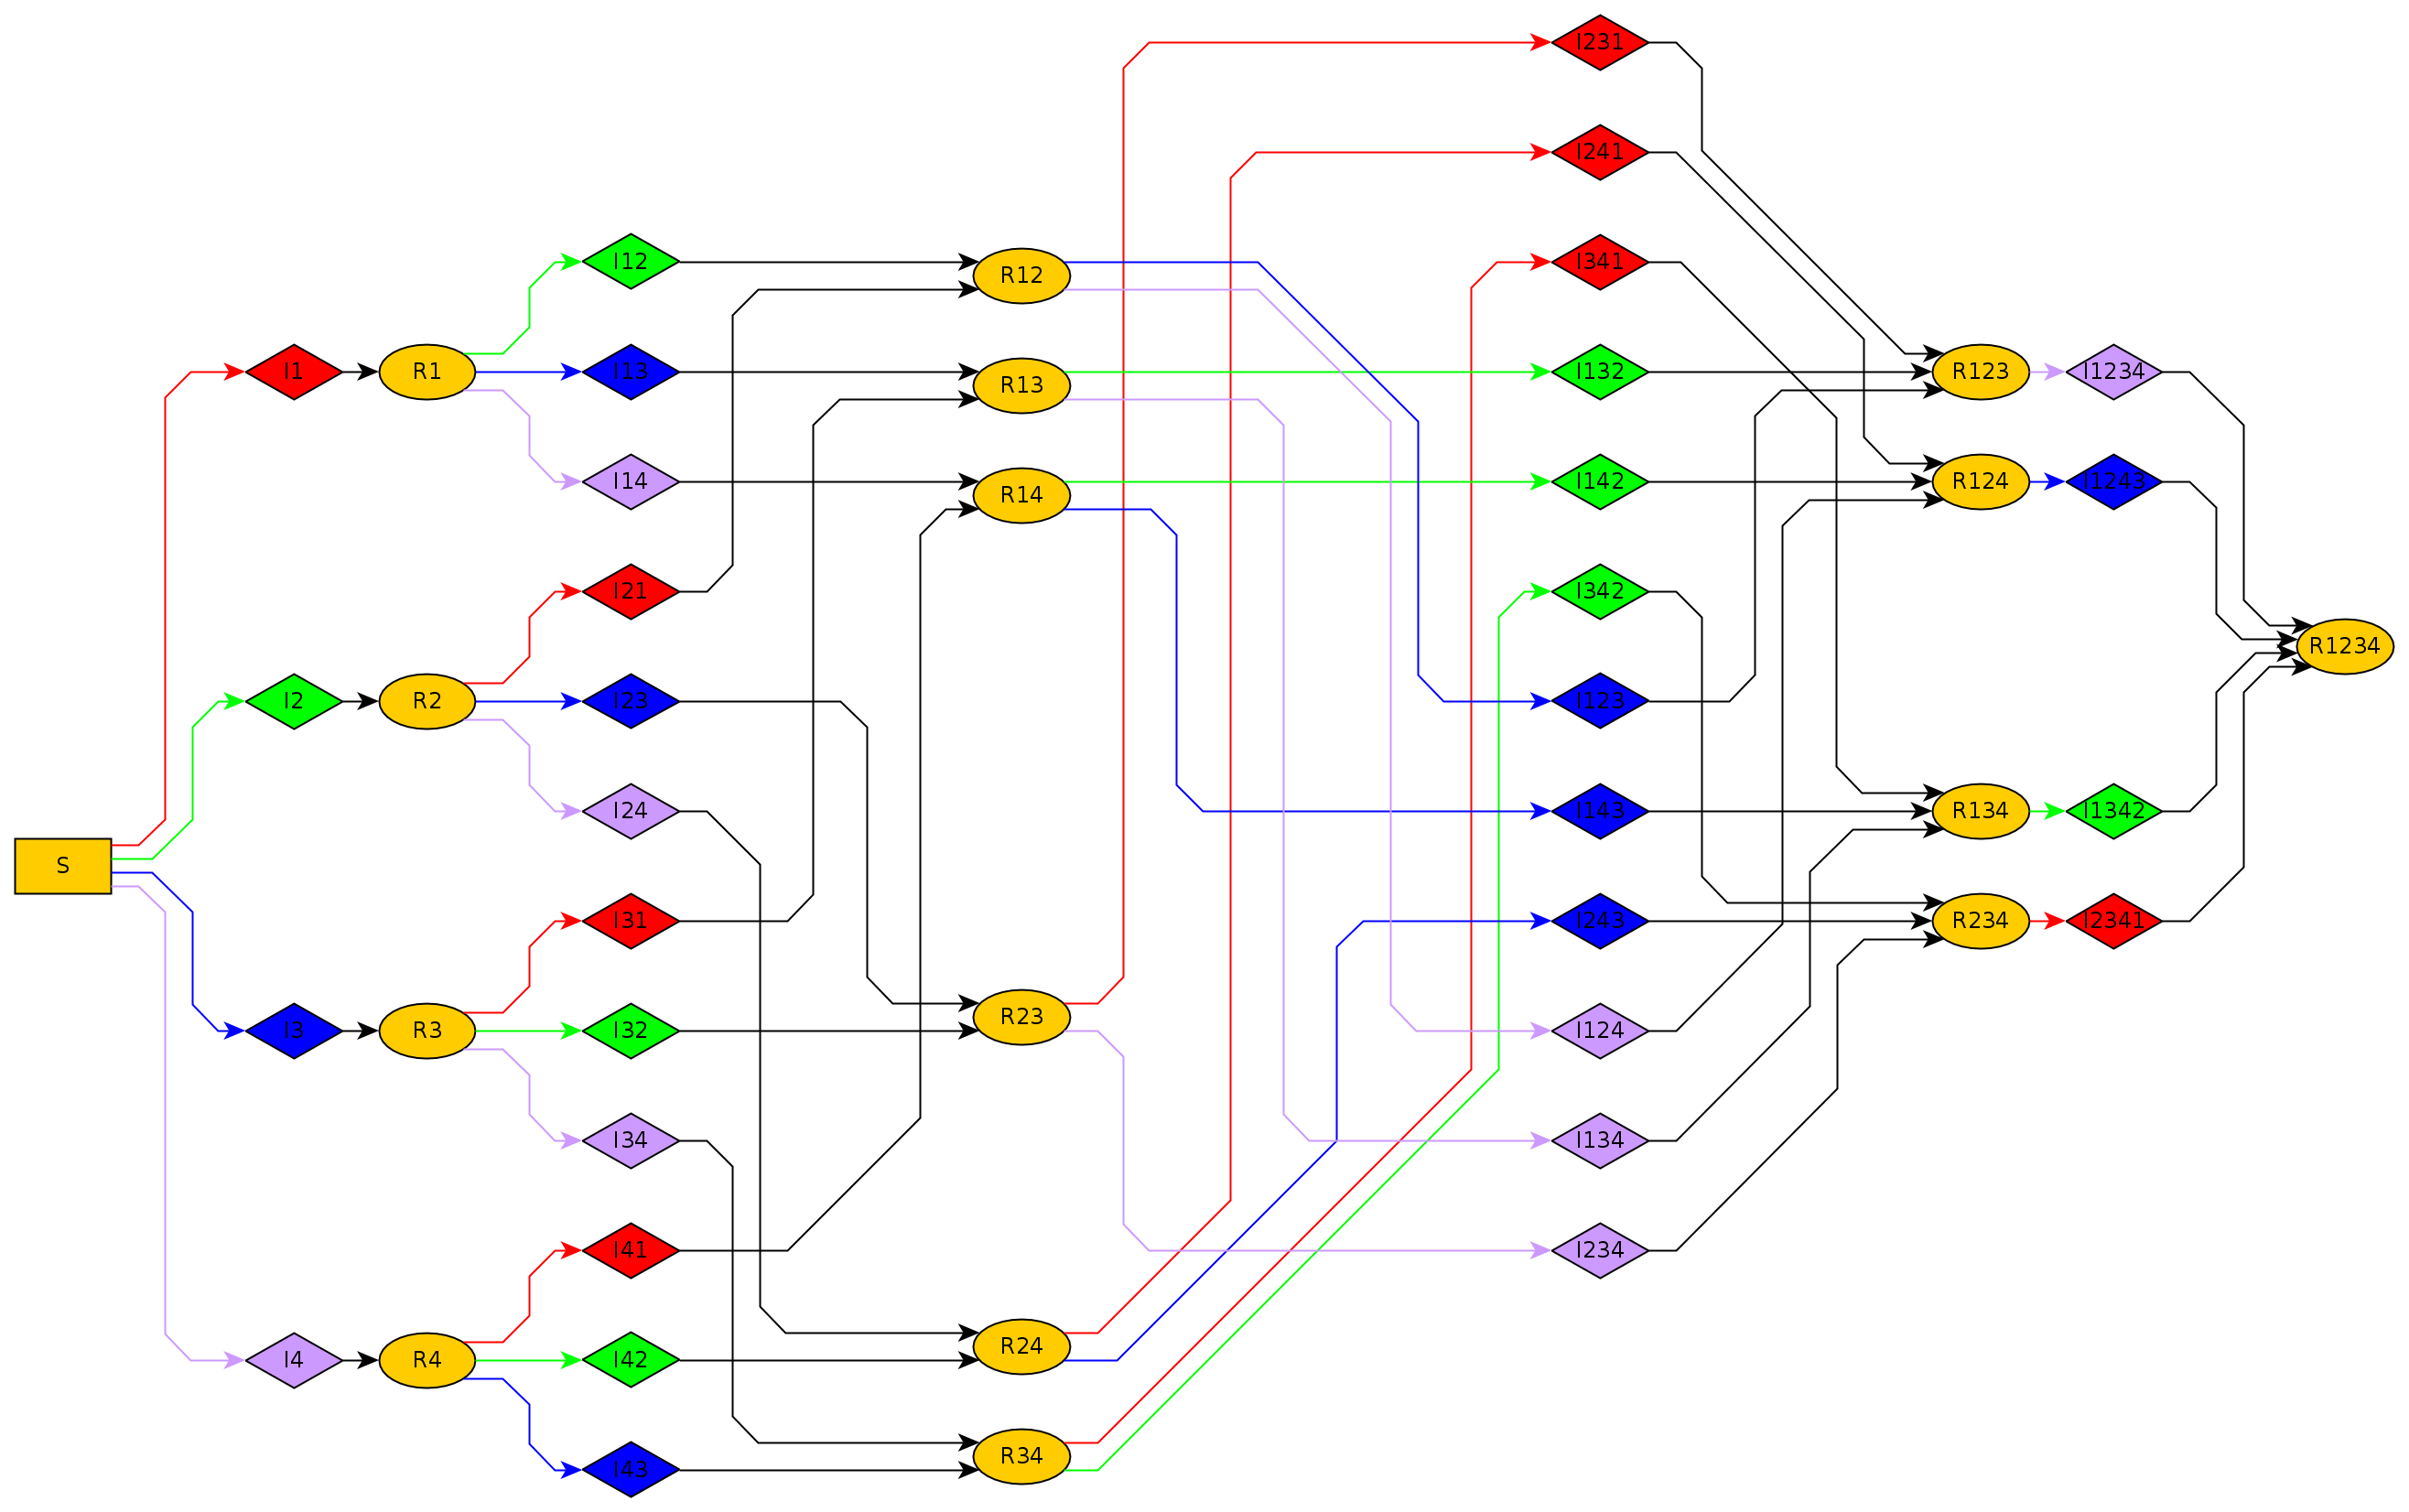
\includegraphics[width=16cm]{Dengue4.png}

 \caption{Block diagram detailing the stochastic model. Infected individuals 
with different Dengue viruses are represented by different colors. Infections 
are also represented by colored arrows matching the virus type.}
 \label{fig:sde_blocks}
\end{figure}


Where $S$ are individuals susceptible to all 4 types of dengue, $I_i$ 
infectious 
with Dengue type $i$, $R_i$ individuals recovered from Dengue type $i$ and 
$N(t) = S(t) + I_*(t) + R_*(t)$ is the total population size at time $t$. 
Infectious individuals already on their secondary and later Dengue infections 
are represented by indices $\{i,j,k,l\}$ which can take values in the close 
interval $(1,4)$. For example, $I_{[23]1}$ is an individual 
which has had Dengues type 2 and 3 in the past -- and therefore is immune to 
them -- and is currently transmitting Dengue 1. 
The index outside the bracket 
denotes current infection. Recovered individuals indices denote their immunity, 
so for instance $R_{123}$ is an individual which is immune to Dengue types 1, 2 
and 3, but not to 4. Let $I_{*i} = \sum I_{[\ldots]i}$ with $[\ldots]$ 
representing exposure history of the infected individual which can vary from 0 
to 3 in length. 
All individuals are born to the $S$ state and birth and death 
rates are equal.

\subsection*{Stochastic Model}
Let's now assume that $S(t)$, $I_*(t)$ and $R_*(t)$ are random variables 
representing the state of a stochastic process.
The possible state-transitions and their  probabilities are listed in table 
\ref{tab:trans}.

\begin{table}
\caption{
{\bf State-transitions and probabilities: $P(\Delta X(t)|X(t))$}. The 
transitions are summarized below. Fully expanded, the system contemplates 64 
possible state transitions, as can be verified in figure \ref{fig:sde_blocks}. 
$^\dag$: Non-zero elements of $(\Delta X)_i$.
}
\label{tab:trans}
\begin{center}
\begin{tabular}[c]{l|l|l|l|l}
\hline
$i$ & Transition & Probability, $p_i$ & State Change$^\dag$ & Description\\
\hline
$1..4$ & $S \rightarrow I_i$ & $\beta S I_{*i} \Delta t$ & $\Delta S(t)=-1,\, 
\Delta I_i(t) = 1$ & Primary infection \\
$5..8$ & $I_i \rightarrow R_i$ & $\sigma I_i \Delta t$ & $\Delta I_i(t)=-1,\, 
\Delta R_i(t) = 1$ & Primary recovery\\
$9..20$ & $R_i \rightarrow I_{[i]j}$ & $\beta \delta R_i I_{*j}\Delta t$ & 
$\Delta R_i(t)=-1,\, \Delta I_{[i]j}(t) = 1$ & Secondary infection\\
$21..32$ & $I_{[i]j} \rightarrow R_{ij}$ & $\sigma I_{[i]j}\Delta t$ &$\Delta 
I_{[i]j}(t)=-1,\, \Delta R_{ij}(t) = 1$& Secondary recovery\\
$33..44$ & $R_{ij} \rightarrow I_{[ij]k}$ & $\beta \delta R_{ij} I_{*k}\Delta 
t$ & $\Delta R_{ij}(t)=-1,\, \Delta I_{[ij]k}(t) = 1$& Tertiary infection\\
$45..56$ & $I_{[ij]k} \rightarrow R_{ijk}$ & $\sigma I_{[ij]k}\Delta t$ 
& $\Delta I_{[ij]k}(t)=-1,\, \Delta R_{ijk}(t) = 1$& Tertiary recovery\\
$57..60$ & $R_{ijk} \rightarrow I_{[ijk]l}$ & $\beta \delta R_{ijk} 
I_{*l}\Delta t$ & $\Delta R_{ijk}(t)=-1,\, \Delta I_{[ijk]l}(t) = 1$& Quaternary 
infection\\
$61..64$ & $I_{[ijk]l} \rightarrow R_{ijkl}$ & $\sigma I_{[ijk]l}\Delta t$ & 
$\Delta 
I_{[ijk]l}(t)=-1,\, \Delta R_{ijkl}(t) = 1$ & Quaternary recovery\\
$65$ & $\rightarrow S$ & $\mu N\Delta t$ & $\Delta S = 1$ & Birth\\
$66..113$ & $All \rightarrow$ & $\mu N\Delta t$ & $\Delta S = \Delta I_* = 
\Delta R_* = -1$ & Death\\
$114$ & No transition & $1-\sum_i p_i$ & No change & ---\\
\hline
\end{tabular}
\end{center}

\end{table}

The stochastic model can be described as a continuous time Markov jump process. 
Let
$$\overrightarrow{X}(t) = [S(t), I_1(t), I_2(t), \ldots, R_{1234}(t)]$$ 
be the 
state of the system at the time $t$. $\sum X(t) = N, \forall t$ with $N$ being 
the population size. 
The system is written as a forward Kolmogorov differential equation, which in 
matrix form looks like
\begin{equation}
\frac{dp_i(t)}{dt} = Q p_i(t) 
\end{equation}

Where $p_i(t)$ is  the vector of transition probabilities (given in table 
\ref{tab:trans}) and Q is the generator matrix, whose  values represent the 
transition rates between all possible states of the system. The full formula 
and matrices are ommited due to their large sizes.

The model can also represented as a system of Itô stochastic differential 
equations. To derive the equivalent system of Itô SDEs, we follow the procedure 
of \citet{allen_modeling_2007}. 

The procedure starts with the identification of the all the possible 
transitions of the system's state and the probabilities associated with them, 
which we have already done (Table \ref{tab:trans}). The second step is to 
derive the expectation and covariance for these changes.

\subsection*{Expected Change and Covariance Matrix}

It is useful to calculate the expected change and the covariance matrix for the 
changes 
\begin{align*}
 \Delta X = [&\Delta S, \Delta I_1, \Delta I_2, \Delta I_3, \Delta I_4,
 \Delta R_1, \Delta R_2, \Delta R_3, \Delta R_4, \Delta I_{12}, \Delta I_{13}, 
\Delta I_{14},\\
&\Delta I_{21}, \Delta I_{23}, \Delta I_{24}, \Delta I_{31},\Delta I_{32}, 
\Delta I_{34}, \Delta I_{41}, \Delta I_{42}, \Delta I_{43},\\
&\Delta R_{12}, 
\Delta R_{13}, \Delta R_{14}, \Delta R_{23}, \Delta R_{24}, \Delta R_{34},
\Delta I_{231}, \Delta I_{241},\\ 
&\Delta I_{341}, \Delta I_{132}, \Delta I_{142},\Delta I_{342}, \Delta I_{123}, 
\Delta I_{143}, \Delta I_{243}, \Delta I_{124},\\
&\Delta I_{134}, \Delta I_{234}, \Delta R_{123}, \Delta R_{124}, \Delta R_{134},
\Delta R_{234},\\ 
&\Delta I_{1234}, \Delta I_{1243}, \Delta I_{1342},\Delta I_{2341},\Delta 
R_{1234}]^T
\end{align*}

 



Thus from the probabilities of table \ref{tab:trans},

\begin{equation}
 E(\Delta X)=\sum_{i=1}^{114} p_i (\Delta X)_i=
\begin{pmatrix}
-\beta S \sum_{i=1}^4 I_{*1} + \mu N -\mu S\\
\beta S I_{*1} -\sigma I_1 -\mu I_1\\
\vdots\\
\beta S I_{*4} -\sigma I_4 -\mu I_4\\
\sigma I_1 - \beta \delta R_1 \sum_{j\neq 1} I_{*j} -\mu R_1\\
\vdots\\
\sigma I_4 - \beta \delta R_4 \sum_{j\neq 4} I_{*j} -\mu R_4\\
\beta \delta R_i I_{*j} - \sigma I_{[i]j} -\mu I_{[i]j}\\ 
\sigma I_{[i]j} - \beta \delta R_{ij} I_{*k} - \mu R_{ij}\\
\beta \delta R_{ij} I_{*k} -\sigma I_{[ij]k} -\mu I_{[ij]k}\\ 
\sigma I_{[ij]k} - \beta \delta R_{ijk} I_{*l} -\mu R_{ijk}\\
\beta \delta R_{ijk} I_{*l} - \sigma I_{[ijk]l} - \mu I_{[ijk]l} \\
\sigma I_{[ijk]l} - \mu R_{1234}
\end{pmatrix}
 \Delta t
\end{equation}

The expected change, $E(\Delta X)$, is a $48\times 1$ vector. The covariance 
matrix is a $48\times 48$ matrix, $\Sigma(\Delta X)= E([\Delta X][\Delta X]^T) 
=\sum_{i=1}^{114} p_i (\Delta X)_i (\Delta X)_i^T = V \Delta t$ (see 
\citet{allen_modeling_2007} for details).

Itô stochastic differential equations have the following general form:

\begin{equation}
\label{eq:ito1}
 d X(t) = \mu(X(t),t) dt + S(X(t),t) dW(t)
\end{equation}

where $W(t)$ is a $48\times1$ vector of independent Wiener processes. It turns 
out that the 
diffusion matrix $S=\sqrt{V} = \sqrt{\Sigma/\Delta t}$. In order to avoid 
having to write down V to take its square root, we will use an equivalent 
formulation for \ref{eq:ito1}

\begin{equation}
\label{eq:ito2}
 d X(t) = \mu(X(t),t) dt + B(X(t),t) dW^*(t)
\end{equation}

To compute $B$, we must first denote each change in table \ref{tab:trans}, 
$(\Delta X)_i$ as $(\Delta_{1i}, \Delta_{2i}, \ldots, \Delta_{48i})$ which is 
equivalent to writing $(\Delta_{Si}, \Delta_{I_1i}, \ldots, 
\Delta_{R_{1234}i})$, as each component represents the amount and direction 
(sign)  of the change in all state variables. The we can define each $(i,j)$ 
element in matrix B as:

\begin{equation}
 B_{ij} = \Delta_{ij}\sqrt{\frac{p_j}{\Delta t}}
\end{equation}

$B$ is then a $48 \times 113$ matrix, whereas $S$ is a $48 \times 48$ matrix. 
Although $B$ is a larger matrix, its easier to compute as it doesn't require 
taking the square root of a matrix. It can be shown that $B\times B^T = V = 
S^2$.

%\setcounter{MaxMatrixCols}{113}
\begin{tiny}
\begin{sideways}
\begin{minipage}{\textheight}
% \resizebox{\textheight}{!}{%
  \[   
\begin{bmatrix}%{rrrrrrrrrrrrrrrrrrrrrrrrrrrrrrrrrrrrrrrrrrrrrrrrrrrrrrrrrrrrrrrrrrrrrrrrrrrrrrrrrrrrrrrrrrrrrrrrrrrrrrrrrrrrrrrrr}
\left( \sqrt{-I_{a_{1}} S \beta} & \sqrt{-I_{a_{2}} S \beta} & \sqrt{-I_{a_{3}} S \beta} & \sqrt{-I_{a_{4}} S \beta} & 0 & 0 & 0 & 0 & 0 & 0 & 0 & 0 & 0 & 0 & 0 & 0 & 0 & 0 & 0 & 0 & 0 & 0 & 0 & 0 & 0 & 0 & 0 & 0 & 0 & 0 & 0 & 0 & 0 & 0 & 0 & 0 & 0 & 0 & 0 & 0 & 0 & 0 & 0 & 0 & 0 & 0 & 0 & 0 & 0 & 0 & 0 & 0 & 0 & 0 & 0 & 0 & 0 & 0 & 0 & 0 & 0 & 0 & 0 & 0 & \sqrt{\mu N} & \sqrt{-S \mu} & 0 & 0 & 0 & 0 & 0 & 0 & 0 & 0 & 0 & 0 & 0 & 0 & 0 & 0 & 0 & 0 & 0 & 0 & 0 & 0 & 0 & 0 & 0 & 0 & 0 & 0 & 0 & 0 & 0 & 0 & 0 & 0 & 0 & 0 & 0 & 0 & 0 & 0 & 0 & 0 & 0 & 0 & 0 & 0 & 0 & 0 & 0 \\
\sqrt{I_{a_{1}} S \beta} & 0 & 0 & 0 & 0 & 0 & 0 & 0 & 0 & 0 & 0 & 0 & 0 & 0 & 
0 
& 0 & 0 & 0 & 0 & 0 & 0 & 0 & 0 & 0 & 0 & 0 & 0 & 0 & 0 & 0 & 0 & 0 & 0 & 0 & 0 
& 0 & 0 & 0 & 0 & 0 & 0 & 0 & 0 & 0 & 0 & 0 & 0 & 0 & 0 & 0 & 0 & 0 & 0 & 0 & 0 
& 0 & 0 & 0 & 0 & 0 & 0 & 0 & 0 & 0 & 0 & 0 & \sqrt{-I_{1} \mu} & 0 & 0 & 0 & 0 
& 0 & 0 & 0 & 0 & 0 & 0 & 0 & 0 & 0 & 0 & 0 & 0 & 0 & 0 & 0 & 0 & 0 & 0 & 0 & 0 
& 0 & 0 & 0 & 0 & 0 & 0 & 0 & 0 & 0 & 0 & 0 & 0 & 0 & 0 & 0 & 0 & 0 & 0 & 0 & 0 
& 0 & 0 \\
0 & \sqrt{I_{a_{2}} S \beta} & 0 & 0 & 0 & 0 & 0 & 0 & 0 & 0 & 0 & 0 & 0 & 0 & 
0 
& 0 & 0 & 0 & 0 & 0 & 0 & 0 & 0 & 0 & 0 & 0 & 0 & 0 & 0 & 0 & 0 & 0 & 0 & 0 & 0 
& 0 & 0 & 0 & 0 & 0 & 0 & 0 & 0 & 0 & 0 & 0 & 0 & 0 & 0 & 0 & 0 & 0 & 0 & 0 & 0 
& 0 & 0 & 0 & 0 & 0 & 0 & 0 & 0 & 0 & 0 & 0 & 0 & \sqrt{-I_{2} \mu} & 0 & 0 & 0 
& 0 & 0 & 0 & 0 & 0 & 0 & 0 & 0 & 0 & 0 & 0 & 0 & 0 & 0 & 0 & 0 & 0 & 0 & 0 & 0 
& 0 & 0 & 0 & 0 & 0 & 0 & 0 & 0 & 0 & 0 & 0 & 0 & 0 & 0 & 0 & 0 & 0 & 0 & 0 & 0 
& 0 & 0 \\
0 & 0 & \sqrt{I_{a_{3}} S \beta} & 0 & 0 & 0 & 0 & 0 & 0 & 0 & 0 & 0 & 0 & 0 & 
0 
& 0 & 0 & 0 & 0 & 0 & 0 & 0 & 0 & 0 & 0 & 0 & 0 & 0 & 0 & 0 & 0 & 0 & 0 & 0 & 0 
& 0 & 0 & 0 & 0 & 0 & 0 & 0 & 0 & 0 & 0 & 0 & 0 & 0 & 0 & 0 & 0 & 0 & 0 & 0 & 0 
& 0 & 0 & 0 & 0 & 0 & 0 & 0 & 0 & 0 & 0 & 0 & 0 & 0 & \sqrt{-I_{3} \mu} & 0 & 0 
& 0 & 0 & 0 & 0 & 0 & 0 & 0 & 0 & 0 & 0 & 0 & 0 & 0 & 0 & 0 & 0 & 0 & 0 & 0 & 0 
& 0 & 0 & 0 & 0 & 0 & 0 & 0 & 0 & 0 & 0 & 0 & 0 & 0 & 0 & 0 & 0 & 0 & 0 & 0 & 0 
& 0 & 0 \\
0 & 0 & 0 & \sqrt{I_{a_{4}} S \beta} & 0 & 0 & 0 & 0 & 0 & 0 & 0 & 0 & 0 & 0 & 
0 
& 0 & 0 & 0 & 0 & 0 & 0 & 0 & 0 & 0 & 0 & 0 & 0 & 0 & 0 & 0 & 0 & 0 & 0 & 0 & 0 
& 0 & 0 & 0 & 0 & 0 & 0 & 0 & 0 & 0 & 0 & 0 & 0 & 0 & 0 & 0 & 0 & 0 & 0 & 0 & 0 
& 0 & 0 & 0 & 0 & 0 & 0 & 0 & 0 & 0 & 0 & 0 & 0 & 0 & 0 & \sqrt{-I_{4} \mu} & 0 
& 0 & 0 & 0 & 0 & 0 & 0 & 0 & 0 & 0 & 0 & 0 & 0 & 0 & 0 & 0 & 0 & 0 & 0 & 0 & 0 
& 0 & 0 & 0 & 0 & 0 & 0 & 0 & 0 & 0 & 0 & 0 & 0 & 0 & 0 & 0 & 0 & 0 & 0 & 0 & 0 
& 0 & 0 \\
0 & 0 & 0 & 0 & \sqrt{-I_{1} \sigma} & 0 & 0 & 0 & \sqrt{-I_{a_{2}} R_{1} \beta 
\delta} & \sqrt{-I_{a_{3}} R_{1} \beta \delta} & \sqrt{-I_{a_{4}} R_{1} \beta 
\delta} & 0 & 0 & 0 & 0 & 0 & 0 & 0 & 0 & 0 & 0 & 0 & 0 & 0 & 0 & 0 & 0 & 0 & 0 
& 0 & 0 & 0 & 0 & 0 & 0 & 0 & 0 & 0 & 0 & 0 & 0 & 0 & 0 & 0 & 0 & 0 & 0 & 0 & 0 
& 0 & 0 & 0 & 0 & 0 & 0 & 0 & 0 & 0 & 0 & 0 & 0 & 0 & 0 & 0 & 0 & 0 & 0 & 0 & 0 
& 0 & \sqrt{-R_{1} \mu} & 0 & 0 & 0 & 0 & 0 & 0 & 0 & 0 & 0 & 0 & 0 & 0 & 0 & 0 
& 0 & 0 & 0 & 0 & 0 & 0 & 0 & 0 & 0 & 0 & 0 & 0 & 0 & 0 & 0 & 0 & 0 & 0 & 0 & 0 
& 0 & 0 & 0 & 0 & 0 & 0 & 0 & 0 \\
0 & 0 & 0 & 0 & 0 & \sqrt{-I_{2} \sigma} & 0 & 0 & 0 & 0 & 0 & \sqrt{-I_{a_{1}} 
R_{2} \beta \delta} & \sqrt{-I_{a_{3}} R_{2} \beta \delta} & \sqrt{-I_{a_{4}} 
R_{2} \beta \delta} & 0 & 0 & 0 & 0 & 0 & 0 & 0 & 0 & 0 & 0 & 0 & 0 & 0 & 0 & 0 
& 0 & 0 & 0 & 0 & 0 & 0 & 0 & 0 & 0 & 0 & 0 & 0 & 0 & 0 & 0 & 0 & 0 & 0 & 0 & 0 
& 0 & 0 & 0 & 0 & 0 & 0 & 0 & 0 & 0 & 0 & 0 & 0 & 0 & 0 & 0 & 0 & 0 & 0 & 0 & 0 
& 0 & 0 & \sqrt{-R_{2} \mu} & 0 & 0 & 0 & 0 & 0 & 0 & 0 & 0 & 0 & 0 & 0 & 0 & 0 
& 0 & 0 & 0 & 0 & 0 & 0 & 0 & 0 & 0 & 0 & 0 & 0 & 0 & 0 & 0 & 0 & 0 & 0 & 0 & 0 
& 0 & 0 & 0 & 0 & 0 & 0 & 0 & 0 \\
0 & 0 & 0 & 0 & 0 & 0 & \sqrt{-I_{3} \sigma} & 0 & 0 & 0 & 0 & 0 & 0 & 0 & 
\sqrt{-I_{a_{1}} R_{3} \beta \delta} & \sqrt{-I_{a_{2}} R_{3} \beta \delta} & 
\sqrt{-I_{a_{4}} R_{3} \beta \delta} & 0 & 0 & 0 & 0 & 0 & 0 & 0 & 0 & 0 & 0 & 
0 
& 0 & 0 & 0 & 0 & 0 & 0 & 0 & 0 & 0 & 0 & 0 & 0 & 0 & 0 & 0 & 0 & 0 & 0 & 0 & 0 
& 0 & 0 & 0 & 0 & 0 & 0 & 0 & 0 & 0 & 0 & 0 & 0 & 0 & 0 & 0 & 0 & 0 & 0 & 0 & 0 
& 0 & 0 & 0 & 0 & \sqrt{-R_{3} \mu} & 0 & 0 & 0 & 0 & 0 & 0 & 0 & 0 & 0 & 0 & 0 
& 0 & 0 & 0 & 0 & 0 & 0 & 0 & 0 & 0 & 0 & 0 & 0 & 0 & 0 & 0 & 0 & 0 & 0 & 0 & 0 
& 0 & 0 & 0 & 0 & 0 & 0 & 0 & 0 & 0 \\
0 & 0 & 0 & 0 & 0 & 0 & 0 & \sqrt{-I_{4} \sigma} & 0 & 0 & 0 & 0 & 0 & 0 & 0 & 
0 
& 0 & \sqrt{-I_{a_{1}} R_{4} \beta \delta} & \sqrt{-I_{a_{2}} R_{4} \beta 
\delta} & \sqrt{-I_{a_{3}} R_{4} \beta \delta} & 0 & 0 & 0 & 0 & 0 & 0 & 0 & 0 
& 
0 & 0 & 0 & 0 & 0 & 0 & 0 & 0 & 0 & 0 & 0 & 0 & 0 & 0 & 0 & 0 & 0 & 0 & 0 & 0 & 
0 & 0 & 0 & 0 & 0 & 0 & 0 & 0 & 0 & 0 & 0 & 0 & 0 & 0 & 0 & 0 & 0 & 0 & 0 & 0 & 
0 & 0 & 0 & 0 & 0 & \sqrt{-R_{4} \mu} & 0 & 0 & 0 & 0 & 0 & 0 & 0 & 0 & 0 & 0 & 
0 & 0 & 0 & 0 & 0 & 0 & 0 & 0 & 0 & 0 & 0 & 0 & 0 & 0 & 0 & 0 & 0 & 0 & 0 & 0 & 
0 & 0 & 0 & 0 & 0 & 0 & 0 & 0 & 0 \\
0 & 0 & 0 & 0 & \sqrt{I_{1} \sigma} & 0 & 0 & 0 & \sqrt{I_{a_{2}} R_{1} \beta 
\delta} & 0 & 0 & 0 & 0 & 0 & 0 & 0 & 0 & 0 & 0 & 0 & \sqrt{-I_{12} \sigma} & 0 
& 0 & 0 & 0 & 0 & 0 & 0 & 0 & 0 & 0 & 0 & 0 & 0 & 0 & 0 & 0 & 0 & 0 & 0 & 0 & 0 
& 0 & 0 & 0 & 0 & 0 & 0 & 0 & 0 & 0 & 0 & 0 & 0 & 0 & 0 & 0 & 0 & 0 & 0 & 0 & 0 
& 0 & 0 & 0 & 0 & 0 & 0 & 0 & 0 & 0 & 0 & 0 & 0 & \sqrt{-I_{12} \mu} & 0 & 0 & 
0 
& 0 & 0 & 0 & 0 & 0 & 0 & 0 & 0 & 0 & 0 & 0 & 0 & 0 & 0 & 0 & 0 & 0 & 0 & 0 & 0 
& 0 & 0 & 0 & 0 & 0 & 0 & 0 & 0 & 0 & 0 & 0 & 0 & 0 & 0 & 0 \\
0 & 0 & 0 & 0 & 0 & \sqrt{I_{2} \sigma} & 0 & 0 & 0 & \sqrt{I_{a_{3}} R_{1} 
\beta \delta} & 0 & 0 & 0 & 0 & 0 & 0 & 0 & 0 & 0 & 0 & 0 & \sqrt{-I_{13} 
\sigma} & 0 & 0 & 0 & 0 & 0 & 0 & 0 & 0 & 0 & 0 & 0 & 0 & 0 & 0 & 0 & 0 & 0 & 0 
& 0 & 0 & 0 & 0 & 0 & 0 & 0 & 0 & 0 & 0 & 0 & 0 & 0 & 0 & 0 & 0 & 0 & 0 & 0 & 0 
& 0 & 0 & 0 & 0 & 0 & 0 & 0 & 0 & 0 & 0 & 0 & 0 & 0 & 0 & 0 & \sqrt{-I_{13} 
\mu} 
& 0 & 0 & 0 & 0 & 0 & 0 & 0 & 0 & 0 & 0 & 0 & 0 & 0 & 0 & 0 & 0 & 0 & 0 & 0 & 0 
& 0 & 0 & 0 & 0 & 0 & 0 & 0 & 0 & 0 & 0 & 0 & 0 & 0 & 0 & 0 & 0 & 0 \\
0 & 0 & 0 & 0 & 0 & 0 & \sqrt{I_{3} \sigma} & 0 & 0 & 0 & \sqrt{I_{a_{4}} R_{1} 
\beta \delta} & 0 & 0 & 0 & 0 & 0 & 0 & 0 & 0 & 0 & 0 & 0 & \sqrt{-I_{14} 
\sigma} & 0 & 0 & 0 & 0 & 0 & 0 & 0 & 0 & 0 & 0 & 0 & 0 & 0 & 0 & 0 & 0 & 0 & 0 
& 0 & 0 & 0 & 0 & 0 & 0 & 0 & 0 & 0 & 0 & 0 & 0 & 0 & 0 & 0 & 0 & 0 & 0 & 0 & 0 
& 0 & 0 & 0 & 0 & 0 & 0 & 0 & 0 & 0 & 0 & 0 & 0 & 0 & 0 & 0 & \sqrt{-I_{14} 
\mu} 
& 0 & 0 & 0 & 0 & 0 & 0 & 0 & 0 & 0 & 0 & 0 & 0 & 0 & 0 & 0 & 0 & 0 & 0 & 0 & 0 
& 0 & 0 & 0 & 0 & 0 & 0 & 0 & 0 & 0 & 0 & 0 & 0 & 0 & 0 & 0 & 0 \\
0 & 0 & 0 & 0 & 0 & 0 & 0 & \sqrt{I_{4} \sigma} & 0 & 0 & 0 & \sqrt{I_{a_{1}} 
R_{2} \beta \delta} & 0 & 0 & 0 & 0 & 0 & 0 & 0 & 0 & 0 & 0 & 0 & \sqrt{-I_{21} 
\sigma} & 0 & 0 & 0 & 0 & 0 & 0 & 0 & 0 & 0 & 0 & 0 & 0 & 0 & 0 & 0 & 0 & 0 & 0 
& 0 & 0 & 0 & 0 & 0 & 0 & 0 & 0 & 0 & 0 & 0 & 0 & 0 & 0 & 0 & 0 & 0 & 0 & 0 & 0 
& 0 & 0 & 0 & 0 & 0 & 0 & 0 & 0 & 0 & 0 & 0 & 0 & 0 & 0 & 0 & \sqrt{-I_{21} 
\mu} 
& 0 & 0 & 0 & 0 & 0 & 0 & 0 & 0 & 0 & 0 & 0 & 0 & 0 & 0 & 0 & 0 & 0 & 0 & 0 & 0 
& 0 & 0 & 0 & 0 & 0 & 0 & 0 & 0 & 0 & 0 & 0 & 0 & 0 & 0 & 0 \\
0 & 0 & 0 & 0 & 0 & 0 & 0 & 0 & 0 & 0 & 0 & 0 & \sqrt{I_{a_{3}} R_{2} \beta 
\delta} & 0 & 0 & 0 & 0 & 0 & 0 & 0 & 0 & 0 & 0 & 0 & \sqrt{-I_{23} \sigma} & 0 
& 0 & 0 & 0 & 0 & 0 & 0 & 0 & 0 & 0 & 0 & 0 & 0 & 0 & 0 & 0 & 0 & 0 & 0 & 0 & 0 
& 0 & 0 & 0 & 0 & 0 & 0 & 0 & 0 & 0 & 0 & 0 & 0 & 0 & 0 & 0 & 0 & 0 & 0 & 0 & 0 
& 0 & 0 & 0 & 0 & 0 & 0 & 0 & 0 & 0 & 0 & 0 & 0 & \sqrt{-I_{23} \mu} & 0 & 0 & 
0 
& 0 & 0 & 0 & 0 & 0 & 0 & 0 & 0 & 0 & 0 & 0 & 0 & 0 & 0 & 0 & 0 & 0 & 0 & 0 & 0 
& 0 & 0 & 0 & 0 & 0 & 0 & 0 & 0 & 0 & 0 & 0 \\
0 & 0 & 0 & 0 & 0 & 0 & 0 & 0 & 0 & 0 & 0 & 0 & 0 & \sqrt{I_{a_{4}} R_{2} \beta 
\delta} & 0 & 0 & 0 & 0 & 0 & 0 & 0 & 0 & 0 & 0 & 0 & \sqrt{-I_{24} \sigma} & 0 
& 0 & 0 & 0 & 0 & 0 & 0 & 0 & 0 & 0 & 0 & 0 & 0 & 0 & 0 & 0 & 0 & 0 & 0 & 0 & 0 
& 0 & 0 & 0 & 0 & 0 & 0 & 0 & 0 & 0 & 0 & 0 & 0 & 0 & 0 & 0 & 0 & 0 & 0 & 0 & 0 
& 0 & 0 & 0 & 0 & 0 & 0 & 0 & 0 & 0 & 0 & 0 & 0 & \sqrt{-I_{24} \mu} & 0 & 0 & 
0 
& 0 & 0 & 0 & 0 & 0 & 0 & 0 & 0 & 0 & 0 & 0 & 0 & 0 & 0 & 0 & 0 & 0 & 0 & 0 & 0 
& 0 & 0 & 0 & 0 & 0 & 0 & 0 & 0 & 0 & 0 \\
0 & 0 & 0 & 0 & 0 & 0 & 0 & 0 & 0 & 0 & 0 & 0 & 0 & 0 & \sqrt{I_{a_{1}} R_{3} 
\beta \delta} & 0 & 0 & 0 & 0 & 0 & 0 & 0 & 0 & 0 & 0 & 0 & \sqrt{-I_{31} 
\sigma} & 0 & 0 & 0 & 0 & 0 & 0 & 0 & 0 & 0 & 0 & 0 & 0 & 0 & 0 & 0 & 0 & 0 & 0 
& 0 & 0 & 0 & 0 & 0 & 0 & 0 & 0 & 0 & 0 & 0 & 0 & 0 & 0 & 0 & 0 & 0 & 0 & 0 & 0 
& 0 & 0 & 0 & 0 & 0 & 0 & 0 & 0 & 0 & 0 & 0 & 0 & 0 & 0 & 0 & \sqrt{-I_{31} 
\mu} 
& 0 & 0 & 0 & 0 & 0 & 0 & 0 & 0 & 0 & 0 & 0 & 0 & 0 & 0 & 0 & 0 & 0 & 0 & 0 & 0 
& 0 & 0 & 0 & 0 & 0 & 0 & 0 & 0 & 0 & 0 & 0 & 0 \\
0 & 0 & 0 & 0 & 0 & 0 & 0 & 0 & 0 & 0 & 0 & 0 & 0 & 0 & 0 & \sqrt{I_{a_{2}} 
R_{3} \beta \delta} & 0 & 0 & 0 & 0 & 0 & 0 & 0 & 0 & 0 & 0 & 0 & \sqrt{-I_{32} 
\sigma} & 0 & 0 & 0 & 0 & 0 & 0 & 0 & 0 & 0 & 0 & 0 & 0 & 0 & 0 & 0 & 0 & 0 & 0 
& 0 & 0 & 0 & 0 & 0 & 0 & 0 & 0 & 0 & 0 & 0 & 0 & 0 & 0 & 0 & 0 & 0 & 0 & 0 & 0 
& 0 & 0 & 0 & 0 & 0 & 0 & 0 & 0 & 0 & 0 & 0 & 0 & 0 & 0 & 0 & \sqrt{-I_{32} 
\mu} 
& 0 & 0 & 0 & 0 & 0 & 0 & 0 & 0 & 0 & 0 & 0 & 0 & 0 & 0 & 0 & 0 & 0 & 0 & 0 & 0 
& 0 & 0 & 0 & 0 & 0 & 0 & 0 & 0 & 0 & 0 & 0 \\
0 & 0 & 0 & 0 & 0 & 0 & 0 & 0 & 0 & 0 & 0 & 0 & 0 & 0 & 0 & 0 & \sqrt{I_{a_{4}} 
R_{3} \beta \delta} & 0 & 0 & 0 & 0 & 0 & 0 & 0 & 0 & 0 & 0 & 0 & \sqrt{-I_{34} 
\sigma} & 0 & 0 & 0 & 0 & 0 & 0 & 0 & 0 & 0 & 0 & 0 & 0 & 0 & 0 & 0 & 0 & 0 & 0 
& 0 & 0 & 0 & 0 & 0 & 0 & 0 & 0 & 0 & 0 & 0 & 0 & 0 & 0 & 0 & 0 & 0 & 0 & 0 & 0 
& 0 & 0 & 0 & 0 & 0 & 0 & 0 & 0 & 0 & 0 & 0 & 0 & 0 & 0 & 0 & \sqrt{-I_{34} 
\mu} 
& 0 & 0 & 0 & 0 & 0 & 0 & 0 & 0 & 0 & 0 & 0 & 0 & 0 & 0 & 0 & 0 & 0 & 0 & 0 & 0 
& 0 & 0 & 0 & 0 & 0 & 0 & 0 & 0 & 0 & 0 \\
0 & 0 & 0 & 0 & 0 & 0 & 0 & 0 & 0 & 0 & 0 & 0 & 0 & 0 & 0 & 0 & 0 & 
\sqrt{I_{a_{1}} R_{4} \beta \delta} & 0 & 0 & 0 & 0 & 0 & 0 & 0 & 0 & 0 & 0 & 0 
& \sqrt{-I_{41} \sigma} & 0 & 0 & 0 & 0 & 0 & 0 & 0 & 0 & 0 & 0 & 0 & 0 & 0 & 0 
& 0 & 0 & 0 & 0 & 0 & 0 & 0 & 0 & 0 & 0 & 0 & 0 & 0 & 0 & 0 & 0 & 0 & 0 & 0 & 0 
& 0 & 0 & 0 & 0 & 0 & 0 & 0 & 0 & 0 & 0 & 0 & 0 & 0 & 0 & 0 & 0 & 0 & 0 & 0 & 
\sqrt{-I_{41} \mu} & 0 & 0 & 0 & 0 & 0 & 0 & 0 & 0 & 0 & 0 & 0 & 0 & 0 & 0 & 0 
& 
0 & 0 & 0 & 0 & 0 & 0 & 0 & 0 & 0 & 0 & 0 & 0 & 0 & 0 \\
0 & 0 & 0 & 0 & 0 & 0 & 0 & 0 & 0 & 0 & 0 & 0 & 0 & 0 & 0 & 0 & 0 & 0 & 
\sqrt{I_{a_{2}} R_{4} \beta \delta} & 0 & 0 & 0 & 0 & 0 & 0 & 0 & 0 & 0 & 0 & 0 
& \sqrt{-I_{42} \sigma} & 0 & 0 & 0 & 0 & 0 & 0 & 0 & 0 & 0 & 0 & 0 & 0 & 0 & 0 
& 0 & 0 & 0 & 0 & 0 & 0 & 0 & 0 & 0 & 0 & 0 & 0 & 0 & 0 & 0 & 0 & 0 & 0 & 0 & 0 
& 0 & 0 & 0 & 0 & 0 & 0 & 0 & 0 & 0 & 0 & 0 & 0 & 0 & 0 & 0 & 0 & 0 & 0 & 0 & 
\sqrt{-I_{42} \mu} & 0 & 0 & 0 & 0 & 0 & 0 & 0 & 0 & 0 & 0 & 0 & 0 & 0 & 0 & 0 
& 
0 & 0 & 0 & 0 & 0 & 0 & 0 & 0 & 0 & 0 & 0 & 0 & 0 \\
0 & 0 & 0 & 0 & 0 & 0 & 0 & 0 & 0 & 0 & 0 & 0 & 0 & 0 & 0 & 0 & 0 & 0 & 0 & 
\sqrt{I_{a_{3}} R_{4} \beta \delta} & 0 & 0 & 0 & 0 & 0 & 0 & 0 & 0 & 0 & 0 & 0 
& \sqrt{-I_{43} \sigma} & 0 & 0 & 0 & 0 & 0 & 0 & 0 & 0 & 0 & 0 & 0 & 0 & 0 & 0 
& 0 & 0 & 0 & 0 & 0 & 0 & 0 & 0 & 0 & 0 & 0 & 0 & 0 & 0 & 0 & 0 & 0 & 0 & 0 & 0 
& 0 & 0 & 0 & 0 & 0 & 0 & 0 & 0 & 0 & 0 & 0 & 0 & 0 & 0 & 0 & 0 & 0 & 0 & 0 & 
\sqrt{-I_{43} \mu} & 0 & 0 & 0 & 0 & 0 & 0 & 0 & 0 & 0 & 0 & 0 & 0 & 0 & 0 & 0 
& 
0 & 0 & 0 & 0 & 0 & 0 & 0 & 0 & 0 & 0 & 0 & 0 \\
0 & 0 & 0 & 0 & 0 & 0 & 0 & 0 & 0 & 0 & 0 & 0 & 0 & 0 & 0 & 0 & 0 & 0 & 0 & 0 & 
\sqrt{I_{12} \sigma} & 0 & 0 & \sqrt{I_{21} \sigma} & 0 & 0 & 0 & 0 & 0 & 0 & 0 
& 0 & 0 & 0 & 0 & 0 & 0 & 0 & \sqrt{-I_{a_{3}} R_{12} \beta \delta} & 0 & 0 & 
\sqrt{-I_{a_{4}} R_{12} \beta \delta} & 0 & 0 & 0 & 0 & 0 & 0 & 0 & 0 & 0 & 0 & 
0 & 0 & 0 & 0 & 0 & 0 & 0 & 0 & 0 & 0 & 0 & 0 & 0 & 0 & 0 & 0 & 0 & 0 & 0 & 0 & 
0 & 0 & 0 & 0 & 0 & 0 & 0 & 0 & 0 & 0 & 0 & 0 & 0 & 0 & \sqrt{-R_{12} \mu} & 0 
& 
0 & 0 & 0 & 0 & 0 & 0 & 0 & 0 & 0 & 0 & 0 & 0 & 0 & 0 & 0 & 0 & 0 & 0 & 0 & 0 & 
0 & 0 & 0 & 0 & 0 \\
0 & 0 & 0 & 0 & 0 & 0 & 0 & 0 & 0 & 0 & 0 & 0 & 0 & 0 & 0 & 0 & 0 & 0 & 0 & 0 & 
0 & \sqrt{I_{13} \sigma} & 0 & 0 & 0 & 0 & \sqrt{I_{31} \sigma} & 0 & 0 & 0 & 0 
& 0 & 0 & 0 & 0 & \sqrt{-I_{a_{2}} R_{13} \beta \delta} & 0 & 0 & 0 & 0 & 0 & 0 
& \sqrt{-I_{a_{4}} R_{13} \beta \delta} & 0 & 0 & 0 & 0 & 0 & 0 & 0 & 0 & 0 & 0 
& 0 & 0 & 0 & 0 & 0 & 0 & 0 & 0 & 0 & 0 & 0 & 0 & 0 & 0 & 0 & 0 & 0 & 0 & 0 & 0 
& 0 & 0 & 0 & 0 & 0 & 0 & 0 & 0 & 0 & 0 & 0 & 0 & 0 & 0 & \sqrt{-R_{13} \mu} & 
0 
& 0 & 0 & 0 & 0 & 0 & 0 & 0 & 0 & 0 & 0 & 0 & 0 & 0 & 0 & 0 & 0 & 0 & 0 & 0 & 0 
& 0 & 0 & 0 & 0 \\
0 & 0 & 0 & 0 & 0 & 0 & 0 & 0 & 0 & 0 & 0 & 0 & 0 & 0 & 0 & 0 & 0 & 0 & 0 & 0 & 
0 & 0 & \sqrt{I_{14} \sigma} & 0 & 0 & 0 & 0 & 0 & 0 & \sqrt{I_{41} \sigma} & 0 
& 0 & 0 & 0 & 0 & 0 & \sqrt{-I_{a_{2}} R_{14} \beta \delta} & 0 & 0 & 
\sqrt{-I_{a_{3}} R_{14} \beta \delta} & 0 & 0 & 0 & 0 & 0 & 0 & 0 & 0 & 0 & 0 & 
0 & 0 & 0 & 0 & 0 & 0 & 0 & 0 & 0 & 0 & 0 & 0 & 0 & 0 & 0 & 0 & 0 & 0 & 0 & 0 & 
0 & 0 & 0 & 0 & 0 & 0 & 0 & 0 & 0 & 0 & 0 & 0 & 0 & 0 & 0 & 0 & 0 & 0 & 
\sqrt{-R_{14} \mu} & 0 & 0 & 0 & 0 & 0 & 0 & 0 & 0 & 0 & 0 & 0 & 0 & 0 & 0 & 0 
& 
0 & 0 & 0 & 0 & 0 & 0 & 0 & 0 & 0 \\
0 & 0 & 0 & 0 & 0 & 0 & 0 & 0 & 0 & 0 & 0 & 0 & 0 & 0 & 0 & 0 & 0 & 0 & 0 & 0 & 
0 & 0 & 0 & 0 & \sqrt{I_{23} \sigma} & 0 & 0 & \sqrt{I_{32} \sigma} & 0 & 0 & 0 
& 0 & \sqrt{-I_{a_{1}} R_{23} \beta \delta} & 0 & 0 & 0 & 0 & 0 & 0 & 0 & 0 & 0 
& 0 & \sqrt{-I_{a_{4}} R_{23} \beta \delta} & 0 & 0 & 0 & 0 & 0 & 0 & 0 & 0 & 0 
& 0 & 0 & 0 & 0 & 0 & 0 & 0 & 0 & 0 & 0 & 0 & 0 & 0 & 0 & 0 & 0 & 0 & 0 & 0 & 0 
& 0 & 0 & 0 & 0 & 0 & 0 & 0 & 0 & 0 & 0 & 0 & 0 & 0 & 0 & 0 & 0 & \sqrt{-R_{23} 
\mu} & 0 & 0 & 0 & 0 & 0 & 0 & 0 & 0 & 0 & 0 & 0 & 0 & 0 & 0 & 0 & 0 & 0 & 0 & 
0 
& 0 & 0 & 0 & 0 \\
0 & 0 & 0 & 0 & 0 & 0 & 0 & 0 & 0 & 0 & 0 & 0 & 0 & 0 & 0 & 0 & 0 & 0 & 0 & 0 & 
0 & 0 & 0 & 0 & 0 & \sqrt{I_{24} \sigma} & 0 & 0 & 0 & 0 & \sqrt{I_{42} \sigma} 
& 0 & 0 & \sqrt{-I_{a_{1}} R_{24} \beta \delta} & 0 & 0 & 0 & 0 & 0 & 0 & 
\sqrt{-I_{a_{3}} R_{24} \beta \delta} & 0 & 0 & 0 & 0 & 0 & 0 & 0 & 0 & 0 & 0 & 
0 & 0 & 0 & 0 & 0 & 0 & 0 & 0 & 0 & 0 & 0 & 0 & 0 & 0 & 0 & 0 & 0 & 0 & 0 & 0 & 
0 & 0 & 0 & 0 & 0 & 0 & 0 & 0 & 0 & 0 & 0 & 0 & 0 & 0 & 0 & 0 & 0 & 0 & 0 & 
\sqrt{-R_{24} \mu} & 0 & 0 & 0 & 0 & 0 & 0 & 0 & 0 & 0 & 0 & 0 & 0 & 0 & 0 & 0 
& 
0 & 0 & 0 & 0 & 0 & 0 & 0 \\
0 & 0 & 0 & 0 & 0 & 0 & 0 & 0 & 0 & 0 & 0 & 0 & 0 & 0 & 0 & 0 & 0 & 0 & 0 & 0 & 
0 & 0 & 0 & 0 & 0 & 0 & 0 & 0 & \sqrt{I_{34} \sigma} & 0 & 0 & \sqrt{I_{43} 
\sigma} & 0 & 0 & \sqrt{-I_{a_{1}} R_{34} \beta \delta} & 0 & 0 & 
\sqrt{-I_{a_{2}} R_{34} \beta \delta} & 0 & 0 & 0 & 0 & 0 & 0 & 0 & 0 & 0 & 0 & 
0 & 0 & 0 & 0 & 0 & 0 & 0 & 0 & 0 & 0 & 0 & 0 & 0 & 0 & 0 & 0 & 0 & 0 & 0 & 0 & 
0 & 0 & 0 & 0 & 0 & 0 & 0 & 0 & 0 & 0 & 0 & 0 & 0 & 0 & 0 & 0 & 0 & 0 & 0 & 0 & 
0 & 0 & 0 & \sqrt{-R_{34} \mu} & 0 & 0 & 0 & 0 & 0 & 0 & 0 & 0 & 0 & 0 & 0 & 0 
& 
0 & 0 & 0 & 0 & 0 & 0 & 0 & 0 & 0 \\
0 & 0 & 0 & 0 & 0 & 0 & 0 & 0 & 0 & 0 & 0 & 0 & 0 & 0 & 0 & 0 & 0 & 0 & 0 & 0 & 
0 & 0 & 0 & 0 & 0 & 0 & 0 & 0 & 0 & 0 & 0 & 0 & \sqrt{I_{a_{1}} R_{23} \beta 
\delta} & 0 & 0 & 0 & 0 & 0 & 0 & 0 & 0 & 0 & 0 & 0 & \sqrt{-I_{231} \sigma} & 
0 
& 0 & 0 & 0 & 0 & 0 & 0 & 0 & 0 & 0 & 0 & 0 & 0 & 0 & 0 & 0 & 0 & 0 & 0 & 0 & 0 
& 0 & 0 & 0 & 0 & 0 & 0 & 0 & 0 & 0 & 0 & 0 & 0 & 0 & 0 & 0 & 0 & 0 & 0 & 0 & 0 
& 0 & 0 & 0 & 0 & 0 & 0 & \sqrt{-I_{231} \mu} & 0 & 0 & 0 & 0 & 0 & 0 & 0 & 0 & 
0 & 0 & 0 & 0 & 0 & 0 & 0 & 0 & 0 & 0 & 0 & 0 \\
0 & 0 & 0 & 0 & 0 & 0 & 0 & 0 & 0 & 0 & 0 & 0 & 0 & 0 & 0 & 0 & 0 & 0 & 0 & 0 & 
0 & 0 & 0 & 0 & 0 & 0 & 0 & 0 & 0 & 0 & 0 & 0 & 0 & \sqrt{I_{a_{1}} R_{24} 
\beta 
\delta} & 0 & 0 & 0 & 0 & 0 & 0 & 0 & 0 & 0 & 0 & 0 & \sqrt{-I_{241} \sigma} & 
0 
& 0 & 0 & 0 & 0 & 0 & 0 & 0 & 0 & 0 & 0 & 0 & 0 & 0 & 0 & 0 & 0 & 0 & 0 & 0 & 0 
& 0 & 0 & 0 & 0 & 0 & 0 & 0 & 0 & 0 & 0 & 0 & 0 & 0 & 0 & 0 & 0 & 0 & 0 & 0 & 0 
& 0 & 0 & 0 & 0 & 0 & 0 & \sqrt{-I_{241} \mu} & 0 & 0 & 0 & 0 & 0 & 0 & 0 & 0 & 
0 & 0 & 0 & 0 & 0 & 0 & 0 & 0 & 0 & 0 & 0 \\
0 & 0 & 0 & 0 & 0 & 0 & 0 & 0 & 0 & 0 & 0 & 0 & 0 & 0 & 0 & 0 & 0 & 0 & 0 & 0 & 
0 & 0 & 0 & 0 & 0 & 0 & 0 & 0 & 0 & 0 & 0 & 0 & 0 & 0 & \sqrt{I_{a_{1}} R_{34} 
\beta \delta} & 0 & 0 & 0 & 0 & 0 & 0 & 0 & 0 & 0 & 0 & 0 & \sqrt{-I_{341} 
\sigma} & 0 & 0 & 0 & 0 & 0 & 0 & 0 & 0 & 0 & 0 & 0 & 0 & 0 & 0 & 0 & 0 & 0 & 0 
& 0 & 0 & 0 & 0 & 0 & 0 & 0 & 0 & 0 & 0 & 0 & 0 & 0 & 0 & 0 & 0 & 0 & 0 & 0 & 0 
& 0 & 0 & 0 & 0 & 0 & 0 & 0 & 0 & 0 & \sqrt{-I_{341} \mu} & 0 & 0 & 0 & 0 & 0 & 
0 & 0 & 0 & 0 & 0 & 0 & 0 & 0 & 0 & 0 & 0 & 0 & 0 \\
0 & 0 & 0 & 0 & 0 & 0 & 0 & 0 & 0 & 0 & 0 & 0 & 0 & 0 & 0 & 0 & 0 & 0 & 0 & 0 & 
0 & 0 & 0 & 0 & 0 & 0 & 0 & 0 & 0 & 0 & 0 & 0 & 0 & 0 & 0 & \sqrt{I_{a_{2}} 
R_{13} \beta \delta} & 0 & 0 & 0 & 0 & 0 & 0 & 0 & 0 & 0 & 0 & 0 & 
\sqrt{-I_{132} \sigma} & 0 & 0 & 0 & 0 & 0 & 0 & 0 & 0 & 0 & 0 & 0 & 0 & 0 & 0 
& 
0 & 0 & 0 & 0 & 0 & 0 & 0 & 0 & 0 & 0 & 0 & 0 & 0 & 0 & 0 & 0 & 0 & 0 & 0 & 0 & 
0 & 0 & 0 & 0 & 0 & 0 & 0 & 0 & 0 & 0 & 0 & 0 & 0 & \sqrt{-I_{132} \mu} & 0 & 0 
& 0 & 0 & 0 & 0 & 0 & 0 & 0 & 0 & 0 & 0 & 0 & 0 & 0 & 0 & 0 \\
0 & 0 & 0 & 0 & 0 & 0 & 0 & 0 & 0 & 0 & 0 & 0 & 0 & 0 & 0 & 0 & 0 & 0 & 0 & 0 & 
0 & 0 & 0 & 0 & 0 & 0 & 0 & 0 & 0 & 0 & 0 & 0 & 0 & 0 & 0 & 0 & \sqrt{I_{a_{2}} 
R_{14} \beta \delta} & 0 & 0 & 0 & 0 & 0 & 0 & 0 & 0 & 0 & 0 & 0 & 
\sqrt{-I_{142} \sigma} & 0 & 0 & 0 & 0 & 0 & 0 & 0 & 0 & 0 & 0 & 0 & 0 & 0 & 0 
& 
0 & 0 & 0 & 0 & 0 & 0 & 0 & 0 & 0 & 0 & 0 & 0 & 0 & 0 & 0 & 0 & 0 & 0 & 0 & 0 & 
0 & 0 & 0 & 0 & 0 & 0 & 0 & 0 & 0 & 0 & 0 & 0 & 0 & \sqrt{-I_{142} \mu} & 0 & 0 
& 0 & 0 & 0 & 0 & 0 & 0 & 0 & 0 & 0 & 0 & 0 & 0 & 0 & 0 \\
0 & 0 & 0 & 0 & 0 & 0 & 0 & 0 & 0 & 0 & 0 & 0 & 0 & 0 & 0 & 0 & 0 & 0 & 0 & 0 & 
0 & 0 & 0 & 0 & 0 & 0 & 0 & 0 & 0 & 0 & 0 & 0 & 0 & 0 & 0 & 0 & 0 & 
\sqrt{I_{a_{2}} R_{34} \beta \delta} & 0 & 0 & 0 & 0 & 0 & 0 & 0 & 0 & 0 & 0 & 
0 
& \sqrt{-I_{342} \sigma} & 0 & 0 & 0 & 0 & 0 & 0 & 0 & 0 & 0 & 0 & 0 & 0 & 0 & 
0 
& 0 & 0 & 0 & 0 & 0 & 0 & 0 & 0 & 0 & 0 & 0 & 0 & 0 & 0 & 0 & 0 & 0 & 0 & 0 & 0 
& 0 & 0 & 0 & 0 & 0 & 0 & 0 & 0 & 0 & 0 & 0 & 0 & 0 & \sqrt{-I_{342} \mu} & 0 & 
0 & 0 & 0 & 0 & 0 & 0 & 0 & 0 & 0 & 0 & 0 & 0 & 0 & 0 \\
0 & 0 & 0 & 0 & 0 & 0 & 0 & 0 & 0 & 0 & 0 & 0 & 0 & 0 & 0 & 0 & 0 & 0 & 0 & 0 & 
0 & 0 & 0 & 0 & 0 & 0 & 0 & 0 & 0 & 0 & 0 & 0 & 0 & 0 & 0 & 0 & 0 & 0 & 
\sqrt{I_{a_{3}} R_{12} \beta \delta} & 0 & 0 & 0 & 0 & 0 & 0 & 0 & 0 & 0 & 0 & 
0 
& \sqrt{-I_{123} \sigma} & 0 & 0 & 0 & 0 & 0 & 0 & 0 & 0 & 0 & 0 & 0 & 0 & 0 & 
0 
& 0 & 0 & 0 & 0 & 0 & 0 & 0 & 0 & 0 & 0 & 0 & 0 & 0 & 0 & 0 & 0 & 0 & 0 & 0 & 0 
& 0 & 0 & 0 & 0 & 0 & 0 & 0 & 0 & 0 & 0 & 0 & 0 & 0 & \sqrt{-I_{123} \mu} & 0 & 
0 & 0 & 0 & 0 & 0 & 0 & 0 & 0 & 0 & 0 & 0 & 0 & 0 \\
0 & 0 & 0 & 0 & 0 & 0 & 0 & 0 & 0 & 0 & 0 & 0 & 0 & 0 & 0 & 0 & 0 & 0 & 0 & 0 & 
0 & 0 & 0 & 0 & 0 & 0 & 0 & 0 & 0 & 0 & 0 & 0 & 0 & 0 & 0 & 0 & 0 & 0 & 0 & 
\sqrt{I_{a_{3}} R_{14} \beta \delta} & 0 & 0 & 0 & 0 & 0 & 0 & 0 & 0 & 0 & 0 & 
0 
& \sqrt{-I_{143} \sigma} & 0 & 0 & 0 & 0 & 0 & 0 & 0 & 0 & 0 & 0 & 0 & 0 & 0 & 
0 
& 0 & 0 & 0 & 0 & 0 & 0 & 0 & 0 & 0 & 0 & 0 & 0 & 0 & 0 & 0 & 0 & 0 & 0 & 0 & 0 
& 0 & 0 & 0 & 0 & 0 & 0 & 0 & 0 & 0 & 0 & 0 & 0 & 0 & \sqrt{-I_{143} \mu} & 0 & 
0 & 0 & 0 & 0 & 0 & 0 & 0 & 0 & 0 & 0 & 0 & 0 \\
0 & 0 & 0 & 0 & 0 & 0 & 0 & 0 & 0 & 0 & 0 & 0 & 0 & 0 & 0 & 0 & 0 & 0 & 0 & 0 & 
0 & 0 & 0 & 0 & 0 & 0 & 0 & 0 & 0 & 0 & 0 & 0 & 0 & 0 & 0 & 0 & 0 & 0 & 0 & 0 & 
\sqrt{I_{a_{3}} R_{24} \beta \delta} & 0 & 0 & 0 & 0 & 0 & 0 & 0 & 0 & 0 & 0 & 
0 
& \sqrt{-I_{243} \sigma} & 0 & 0 & 0 & 0 & 0 & 0 & 0 & 0 & 0 & 0 & 0 & 0 & 0 & 
0 
& 0 & 0 & 0 & 0 & 0 & 0 & 0 & 0 & 0 & 0 & 0 & 0 & 0 & 0 & 0 & 0 & 0 & 0 & 0 & 0 
& 0 & 0 & 0 & 0 & 0 & 0 & 0 & 0 & 0 & 0 & 0 & 0 & 0 & \sqrt{-I_{243} \mu} & 0 & 
0 & 0 & 0 & 0 & 0 & 0 & 0 & 0 & 0 & 0 & 0 \\
0 & 0 & 0 & 0 & 0 & 0 & 0 & 0 & 0 & 0 & 0 & 0 & 0 & 0 & 0 & 0 & 0 & 0 & 0 & 0 & 
0 & 0 & 0 & 0 & 0 & 0 & 0 & 0 & 0 & 0 & 0 & 0 & 0 & 0 & 0 & 0 & 0 & 0 & 0 & 0 & 
0 & \sqrt{I_{a_{4}} R_{12} \beta \delta} & 0 & 0 & 0 & 0 & 0 & 0 & 0 & 0 & 0 & 
0 
& 0 & \sqrt{-I_{124} \sigma} & 0 & 0 & 0 & 0 & 0 & 0 & 0 & 0 & 0 & 0 & 0 & 0 & 
0 
& 0 & 0 & 0 & 0 & 0 & 0 & 0 & 0 & 0 & 0 & 0 & 0 & 0 & 0 & 0 & 0 & 0 & 0 & 0 & 0 
& 0 & 0 & 0 & 0 & 0 & 0 & 0 & 0 & 0 & 0 & 0 & 0 & 0 & 0 & \sqrt{-I_{124} \mu} & 
0 & 0 & 0 & 0 & 0 & 0 & 0 & 0 & 0 & 0 & 0 \\
0 & 0 & 0 & 0 & 0 & 0 & 0 & 0 & 0 & 0 & 0 & 0 & 0 & 0 & 0 & 0 & 0 & 0 & 0 & 0 & 
0 & 0 & 0 & 0 & 0 & 0 & 0 & 0 & 0 & 0 & 0 & 0 & 0 & 0 & 0 & 0 & 0 & 0 & 0 & 0 & 
0 & 0 & \sqrt{I_{a_{4}} R_{13} \beta \delta} & 0 & 0 & 0 & 0 & 0 & 0 & 0 & 0 & 
0 
& 0 & 0 & \sqrt{-I_{134} \sigma} & 0 & 0 & 0 & 0 & 0 & 0 & 0 & 0 & 0 & 0 & 0 & 
0 
& 0 & 0 & 0 & 0 & 0 & 0 & 0 & 0 & 0 & 0 & 0 & 0 & 0 & 0 & 0 & 0 & 0 & 0 & 0 & 0 
& 0 & 0 & 0 & 0 & 0 & 0 & 0 & 0 & 0 & 0 & 0 & 0 & 0 & 0 & 0 & \sqrt{-I_{134} 
\mu} & 0 & 0 & 0 & 0 & 0 & 0 & 0 & 0 & 0 & 0 \\
0 & 0 & 0 & 0 & 0 & 0 & 0 & 0 & 0 & 0 & 0 & 0 & 0 & 0 & 0 & 0 & 0 & 0 & 0 & 0 & 
0 & 0 & 0 & 0 & 0 & 0 & 0 & 0 & 0 & 0 & 0 & 0 & 0 & 0 & 0 & 0 & 0 & 0 & 0 & 0 & 
0 & 0 & 0 & \sqrt{I_{a_{4}} R_{23} \beta \delta} & 0 & 0 & 0 & 0 & 0 & 0 & 0 & 
0 
& 0 & 0 & 0 & \sqrt{-I_{234} \sigma} & 0 & 0 & 0 & 0 & 0 & 0 & 0 & 0 & 0 & 0 & 
0 
& 0 & 0 & 0 & 0 & 0 & 0 & 0 & 0 & 0 & 0 & 0 & 0 & 0 & 0 & 0 & 0 & 0 & 0 & 0 & 0 
& 0 & 0 & 0 & 0 & 0 & 0 & 0 & 0 & 0 & 0 & 0 & 0 & 0 & 0 & 0 & 0 & 
\sqrt{-I_{234} 
\mu} & 0 & 0 & 0 & 0 & 0 & 0 & 0 & 0 & 0 \\
0 & 0 & 0 & 0 & 0 & 0 & 0 & 0 & 0 & 0 & 0 & 0 & 0 & 0 & 0 & 0 & 0 & 0 & 0 & 0 & 
0 & 0 & 0 & 0 & 0 & 0 & 0 & 0 & 0 & 0 & 0 & 0 & 0 & 0 & 0 & 0 & 0 & 0 & 0 & 0 & 
0 & 0 & 0 & 0 & \sqrt{I_{231} \sigma} & 0 & 0 & \sqrt{I_{132} \sigma} & 0 & 0 & 
\sqrt{I_{123} \sigma} & 0 & 0 & 0 & 0 & 0 & \sqrt{-{\left(I_{1234} + I_{124} + 
I_{134} + I_{14} + I_{234} + I_{24} + I_{34} + I_{4}\right)} R_{123} \beta 
\delta} & 0 & 0 & 0 & 0 & 0 & 0 & 0 & 0 & 0 & 0 & 0 & 0 & 0 & 0 & 0 & 0 & 0 & 0 
& 0 & 0 & 0 & 0 & 0 & 0 & 0 & 0 & 0 & 0 & 0 & 0 & 0 & 0 & 0 & 0 & 0 & 0 & 0 & 0 
& 0 & 0 & 0 & 0 & 0 & 0 & 0 & 0 & 0 & \sqrt{-R_{123} \mu} & 0 & 0 & 0 & 0 & 0 & 
0 & 0 & 0 \\
0 & 0 & 0 & 0 & 0 & 0 & 0 & 0 & 0 & 0 & 0 & 0 & 0 & 0 & 0 & 0 & 0 & 0 & 0 & 0 & 
0 & 0 & 0 & 0 & 0 & 0 & 0 & 0 & 0 & 0 & 0 & 0 & 0 & 0 & 0 & 0 & 0 & 0 & 0 & 0 & 
0 & 0 & 0 & 0 & 0 & \sqrt{I_{241} \sigma} & 0 & 0 & \sqrt{I_{142} \sigma} & 0 & 
0 & 0 & 0 & \sqrt{I_{124} \sigma} & 0 & 0 & 0 & \sqrt{-I_{a_{3}} R_{124} \beta 
\delta} & 0 & 0 & 0 & 0 & 0 & 0 & 0 & 0 & 0 & 0 & 0 & 0 & 0 & 0 & 0 & 0 & 0 & 0 
& 0 & 0 & 0 & 0 & 0 & 0 & 0 & 0 & 0 & 0 & 0 & 0 & 0 & 0 & 0 & 0 & 0 & 0 & 0 & 0 
& 0 & 0 & 0 & 0 & 0 & 0 & 0 & 0 & 0 & \sqrt{-R_{124} \mu} & 0 & 0 & 0 & 0 & 0 & 
0 & 0 \\
0 & 0 & 0 & 0 & 0 & 0 & 0 & 0 & 0 & 0 & 0 & 0 & 0 & 0 & 0 & 0 & 0 & 0 & 0 & 0 & 
0 & 0 & 0 & 0 & 0 & 0 & 0 & 0 & 0 & 0 & 0 & 0 & 0 & 0 & 0 & 0 & 0 & 0 & 0 & 0 & 
0 & 0 & 0 & 0 & 0 & 0 & \sqrt{I_{341} \sigma} & 0 & 0 & 0 & 0 & \sqrt{I_{143} 
\sigma} & 0 & 0 & \sqrt{I_{134} \sigma} & 0 & 0 & 0 & \sqrt{-I_{a_{2}} R_{134} 
\beta \delta} & 0 & 0 & 0 & 0 & 0 & 0 & 0 & 0 & 0 & 0 & 0 & 0 & 0 & 0 & 0 & 0 & 
0 & 0 & 0 & 0 & 0 & 0 & 0 & 0 & 0 & 0 & 0 & 0 & 0 & 0 & 0 & 0 & 0 & 0 & 0 & 0 & 
0 & 0 & 0 & 0 & 0 & 0 & 0 & 0 & 0 & 0 & 0 & \sqrt{-R_{134} \mu} & 0 & 0 & 0 & 0 
& 0 & 0 \\
0 & 0 & 0 & 0 & 0 & 0 & 0 & 0 & 0 & 0 & 0 & 0 & 0 & 0 & 0 & 0 & 0 & 0 & 0 & 0 & 
0 & 0 & 0 & 0 & 0 & 0 & 0 & 0 & 0 & 0 & 0 & 0 & 0 & 0 & 0 & 0 & 0 & 0 & 0 & 0 & 
0 & 0 & 0 & 0 & 0 & 0 & 0 & 0 & 0 & \sqrt{I_{342} \sigma} & 0 & 0 & 
\sqrt{I_{243} \sigma} & 0 & 0 & \sqrt{I_{234} \sigma} & 0 & 0 & 0 & 
\sqrt{-I_{a_{1}} R_{234} \beta \delta} & 0 & 0 & 0 & 0 & 0 & 0 & 0 & 0 & 0 & 0 
& 
0 & 0 & 0 & 0 & 0 & 0 & 0 & 0 & 0 & 0 & 0 & 0 & 0 & 0 & 0 & 0 & 0 & 0 & 0 & 0 & 
0 & 0 & 0 & 0 & 0 & 0 & 0 & 0 & 0 & 0 & 0 & 0 & 0 & 0 & 0 & 0 & 0 & 
\sqrt{-R_{234} \mu} & 0 & 0 & 0 & 0 & 0 \\
0 & 0 & 0 & 0 & 0 & 0 & 0 & 0 & 0 & 0 & 0 & 0 & 0 & 0 & 0 & 0 & 0 & 0 & 0 & 0 & 
0 & 0 & 0 & 0 & 0 & 0 & 0 & 0 & 0 & 0 & 0 & 0 & 0 & 0 & 0 & 0 & 0 & 0 & 0 & 0 & 
0 & 0 & 0 & 0 & 0 & 0 & 0 & 0 & 0 & 0 & 0 & 0 & 0 & 0 & 0 & 0 & 
\sqrt{{\left(I_{1234} + I_{124} + I_{134} + I_{14} + I_{234} + I_{24} + I_{34} 
+ 
I_{4}\right)} R_{123} \beta \delta} & 0 & 0 & 0 & \sqrt{-I_{1234} \sigma} & 0 & 
0 & 0 & 0 & 0 & 0 & 0 & 0 & 0 & 0 & 0 & 0 & 0 & 0 & 0 & 0 & 0 & 0 & 0 & 0 & 0 & 
0 & 0 & 0 & 0 & 0 & 0 & 0 & 0 & 0 & 0 & 0 & 0 & 0 & 0 & 0 & 0 & 0 & 0 & 0 & 0 & 
0 & 0 & 0 & 0 & 0 & 0 & \sqrt{-I_{1234} \mu} & 0 & 0 & 0 & 0 \\
0 & 0 & 0 & 0 & 0 & 0 & 0 & 0 & 0 & 0 & 0 & 0 & 0 & 0 & 0 & 0 & 0 & 0 & 0 & 0 & 
0 & 0 & 0 & 0 & 0 & 0 & 0 & 0 & 0 & 0 & 0 & 0 & 0 & 0 & 0 & 0 & 0 & 0 & 0 & 0 & 
0 & 0 & 0 & 0 & 0 & 0 & 0 & 0 & 0 & 0 & 0 & 0 & 0 & 0 & 0 & 0 & 0 & 
\sqrt{I_{a_{3}} R_{124} \beta \delta} & 0 & 0 & 0 & \sqrt{-I_{1243} \sigma} & 0 
& 0 & 0 & 0 & 0 & 0 & 0 & 0 & 0 & 0 & 0 & 0 & 0 & 0 & 0 & 0 & 0 & 0 & 0 & 0 & 0 
& 0 & 0 & 0 & 0 & 0 & 0 & 0 & 0 & 0 & 0 & 0 & 0 & 0 & 0 & 0 & 0 & 0 & 0 & 0 & 0 
& 0 & 0 & 0 & 0 & 0 & 0 & \sqrt{-I_{1243} \mu} & 0 & 0 & 0 \\
0 & 0 & 0 & 0 & 0 & 0 & 0 & 0 & 0 & 0 & 0 & 0 & 0 & 0 & 0 & 0 & 0 & 0 & 0 & 0 & 
0 & 0 & 0 & 0 & 0 & 0 & 0 & 0 & 0 & 0 & 0 & 0 & 0 & 0 & 0 & 0 & 0 & 0 & 0 & 0 & 
0 & 0 & 0 & 0 & 0 & 0 & 0 & 0 & 0 & 0 & 0 & 0 & 0 & 0 & 0 & 0 & 0 & 0 & 
\sqrt{I_{a_{2}} R_{134} \beta \delta} & 0 & 0 & 0 & \sqrt{-I_{1342} \sigma} & 0 
& 0 & 0 & 0 & 0 & 0 & 0 & 0 & 0 & 0 & 0 & 0 & 0 & 0 & 0 & 0 & 0 & 0 & 0 & 0 & 0 
& 0 & 0 & 0 & 0 & 0 & 0 & 0 & 0 & 0 & 0 & 0 & 0 & 0 & 0 & 0 & 0 & 0 & 0 & 0 & 0 
& 0 & 0 & 0 & 0 & 0 & 0 & \sqrt{-I_{1342} \mu} & 0 & 0 \\
0 & 0 & 0 & 0 & 0 & 0 & 0 & 0 & 0 & 0 & 0 & 0 & 0 & 0 & 0 & 0 & 0 & 0 & 0 & 0 & 
0 & 0 & 0 & 0 & 0 & 0 & 0 & 0 & 0 & 0 & 0 & 0 & 0 & 0 & 0 & 0 & 0 & 0 & 0 & 0 & 
0 & 0 & 0 & 0 & 0 & 0 & 0 & 0 & 0 & 0 & 0 & 0 & 0 & 0 & 0 & 0 & 0 & 0 & 0 & 
\sqrt{I_{a_{1}} R_{234} \beta \delta} & 0 & 0 & 0 & \sqrt{-I_{2341} \sigma} & 0 
& 0 & 0 & 0 & 0 & 0 & 0 & 0 & 0 & 0 & 0 & 0 & 0 & 0 & 0 & 0 & 0 & 0 & 0 & 0 & 0 
& 0 & 0 & 0 & 0 & 0 & 0 & 0 & 0 & 0 & 0 & 0 & 0 & 0 & 0 & 0 & 0 & 0 & 0 & 0 & 0 
& 0 & 0 & 0 & 0 & 0 & 0 & \sqrt{-I_{2341} \mu} & 0 \\
0 & 0 & 0 & 0 & 0 & 0 & 0 & 0 & 0 & 0 & 0 & 0 & 0 & 0 & 0 & 0 & 0 & 0 & 0 & 0 & 
0 & 0 & 0 & 0 & 0 & 0 & 0 & 0 & 0 & 0 & 0 & 0 & 0 & 0 & 0 & 0 & 0 & 0 & 0 & 0 & 
0 & 0 & 0 & 0 & 0 & 0 & 0 & 0 & 0 & 0 & 0 & 0 & 0 & 0 & 0 & 0 & 0 & 0 & 0 & 0 & 
\sqrt{I_{1234} \sigma} & \sqrt{I_{1243} \sigma} & \sqrt{I_{1342} \sigma} & 
\sqrt{I_{2341} \sigma} & 0 & 0 & 0 & 0 & 0 & 0 & 0 & 0 & 0 & 0 & 0 & 0 & 0 & 0 
& 
0 & 0 & 0 & 0 & 0 & 0 & 0 & 0 & 0 & 0 & 0 & 0 & 0 & 0 & 0 & 0 & 0 & 0 & 0 & 0 & 
0 & 0 & 0 & 0 & 0 & 0 & 0 & 0 & 0 & 0 & 0 & 0 & 0 & 0 & \sqrt{-R_{1234} \mu}
\end{bmatrix}\right) 
  \]
%}
\end{minipage}

\end{sideways}
\end{tiny}



\section*{Numerical simulations}

There are different approaches to simulate the proposed stochastic  models, the 
Kolmogorov version, can be simulated using Gillespie's algorithm which works 
well for small population sizes but becomes unwieldy for larger populations. 

The SDE version however does not suffer from these scalability issues, with a 
number of solvers available for their simulation
\citep{higham_algorithmic_2001}.

The parameter values used for the numerical simulations can be found on table 

{%
\newcommand{\mc}[3]{\multicolumn{#1}{#2}{#3}}
\begin{table}
\caption{Parameters used for simulations}
\label{tab:pars}
\begin{center}
\begin{tabular}{lcl}
Parameter & Value & Description\\ \hline
$\beta$ & 400/52 & Transmission rate\\
$\delta$ & 0.2 & ×\\
$\sigma$ & \mc{1}{l}{1/1.5} & ×\\
$\mu$ & \mc{1}{l}{$\frac{1}{70\times 52}$} & mortality rate\\
$N$ & \mc{1}{l}{50000} & Population size\\\hline
\end{tabular}
\end{center}
\end{table}
}%


\bibliography{stochd}
\end{document}
